\section{eo\-Deterministic\-Survive\-And\-Die$<$ EOT $>$ Class Template Reference}
\label{classeo_deterministic_survive_and_die}\index{eoDeterministicSurviveAndDie@{eoDeterministicSurviveAndDie}}
An instance (theonly one as of today, Dec.  


{\tt \#include $<$eo\-Survive\-And\-Die.h$>$}

Inheritance diagram for eo\-Deterministic\-Survive\-And\-Die$<$ EOT $>$::\begin{figure}[H]
\begin{center}
\leavevmode
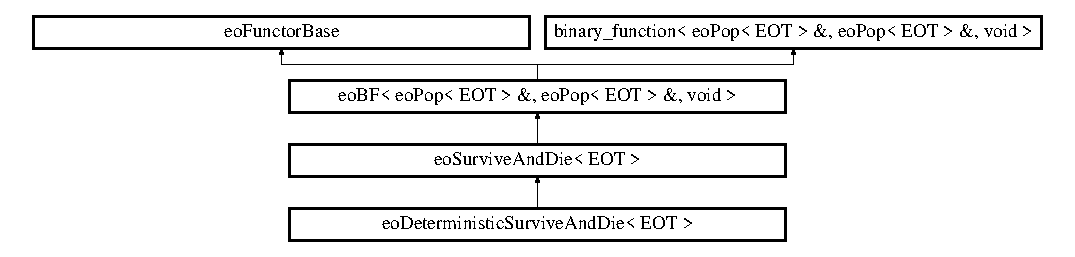
\includegraphics[height=3.01075cm]{classeo_deterministic_survive_and_die}
\end{center}
\end{figure}
\subsection*{Public Member Functions}
\begin{CompactItemize}
\item 
{\bf eo\-Deterministic\-Survive\-And\-Die} (double \_\-survive, double \_\-die, bool \_\-interpret\_\-as\_\-rate=true)\label{classeo_deterministic_survive_and_die_a0}

\begin{CompactList}\small\item\em constructor \item\end{CompactList}\item 
void {\bf operator()} ({\bf eo\-Pop}$<$ {\bf EOT} $>$ \&\_\-pop, {\bf eo\-Pop}$<$ {\bf EOT} $>$ \&\_\-lucky\-Guys)\label{classeo_deterministic_survive_and_die_a1}

\begin{CompactList}\small\item\em The pure virtual function that needs to be implemented by the subclass. \item\end{CompactList}\end{CompactItemize}


\subsection{Detailed Description}
\subsubsection*{template$<$class EOT$>$ class eo\-Deterministic\-Survive\-And\-Die$<$ EOT $>$}

An instance (theonly one as of today, Dec. 

20, 2000) of an {\bf eo\-Survive\-And\-Die}{\rm (p.\,\pageref{classeo_survive_and_die})}, that does everything deterministically

Used in {\bf eo\-Deterministic\-Sa\-DReplacement}{\rm (p.\,\pageref{classeo_deterministic_sa_d_replacement})}. 



Definition at line 73 of file eo\-Survive\-And\-Die.h.

The documentation for this class was generated from the following file:\begin{CompactItemize}
\item 
eo\-Survive\-And\-Die.h\end{CompactItemize}
